% Generated by scripts/build-paper.py — edit paper/src/survey.src.md
\section{Openness and reproducibility}\label{sec:openness-and-reproducibility}

Openness is not a single property (Table 6, Figure 3). Among the 14 core and peripheral studies, code was located in full for 4, in part or as a project page only for 2, and claimed but not located for 2. Weights were located for 1 study, and raw predictions were fully available for 1. The two studies whose code and per-item data are claimed but unlocated could not be matched to a public package \citep{arxiv2609_26758,arxiv2609_26550}. Data restrictions are sometimes legitimate: crash narratives cannot be redistributed under their data agreement \citep{arxiv2609_24052}. The best recomputable case is the CSS replication package with complete per-call records \citep{arxiv2609_24574}. Among repositories, weights and inference code are common for open models; training code, evaluation data and raw predictions are not. Licence fields reported by GitHub as \texttt{NOASSERTION} mean “not identified”, not “no licence”. We record “not located” rather than “absent” throughout.

\begin{figure}[tbp]
\centering
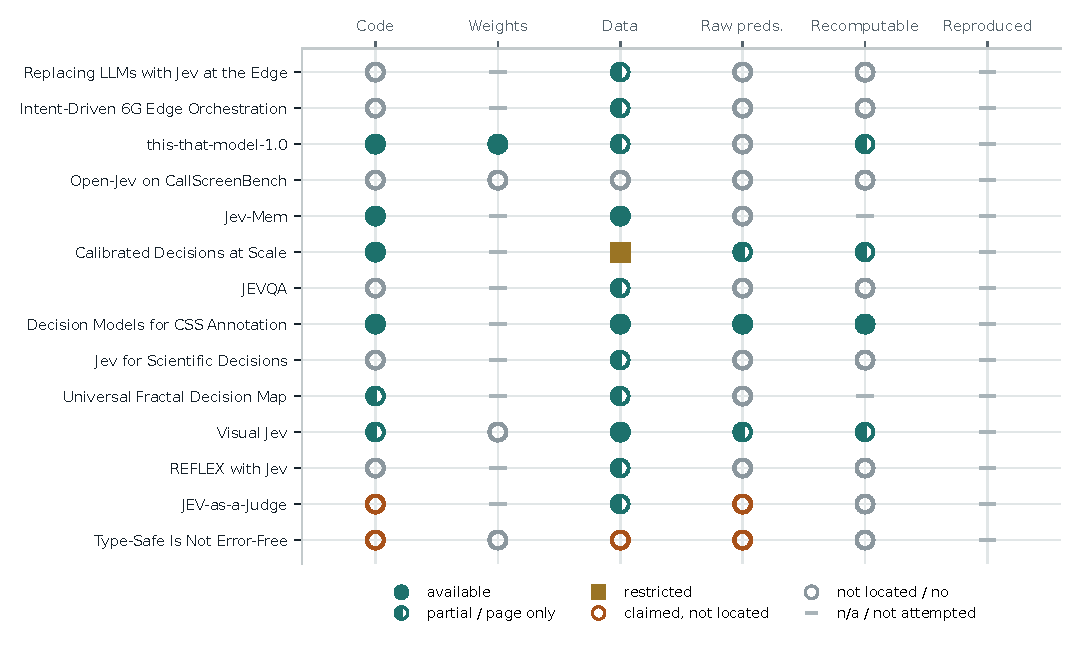
\includegraphics[width=\linewidth]{figures/openness.pdf}
\caption{Openness of the core and peripheral studies across six independent fields.}\label{fig:openness}
\end{figure}

\begin{table}[tbp]
\centering\footnotesize
\caption{Openness of core and peripheral studies: six separate fields (“not located” is not “absent”).}\label{tab:openness}
\begin{tabularx}{\linewidth}{Xllllll}
\toprule
\textbf{Study} & \textbf{Code} & \textbf{Weights} & \textbf{Data} & \textbf{Predictions} & \textbf{Recomputable} & \textbf{Reproduced} \\
\midrule
Replacing LLMs with Jev at the Edge & not located & n/a & partial & not located & no & no \\
Intent-Driven 6G Edge Orchestration & not located & n/a & partial & not located & no & no \\
this-that-model-1.0 & available & available & partial & not located & partial & no \\
Open-Jev on CallScreenBench & not located & not located & not located & not located & no & no \\
Jev-Mem & available & n/a & available & not located & · & no \\
Calibrated Decisions at Scale & available & n/a & restricted & partial & partial & no \\
JEVQA & not located & n/a & partial & not located & no & no \\
Decision Models for CSS Annotation & available & n/a & available & available & available & no \\
Jev for Scientific Decisions & not located & n/a & partial & not located & no & no \\
Universal Fractal Decision Map & partial & n/a & partial & not located & · & no \\
Visual Jev & page only & not located & available & partial & partial & no \\
REFLEX with Jev & not located & n/a & partial & not located & no & no \\
JEV-as-a-Judge & claimed & n/a & partial & claimed & no & no \\
Type-Safe Is Not Error-Free & claimed & not located & claimed & claimed & no & no \\
\bottomrule
\end{tabularx}
\end{table}
